\documentclass{article}
\usepackage{graphicx}
\usepackage[top=1.00in, bottom=1.0in, left=1in, right=1in]{geometry}
\usepackage{outlines}
\usepackage{enumitem}
\setenumerate[1]{label=\Roman*.}
\setenumerate[2]{label=\Alph*.}
\setenumerate[3]{label=\roman*.}
\setenumerate[4]{label=\alph*.}
\title {Operation Manual}
\begin{document}
\maketitle
\begin{outline}[enumerate]

\1 {Device Setup}
\begin{enumerate}
	\item Turn on the Jetson by plugging the power port in. See Figure \ref{fig:jetson1}.
	\item Turn on the motor controller with the switch. See Figure \ref{fig:controller3}.
	\item Turn on the power supply with the switch. See Figure \ref{fig:power1}.
	\item Ensure everything is plugged in correctly. 
        \begin{enumerate}
        \item USB ring light is powered. It's best NOT to power it with the USB ports on the Jetson.
        \item Jetson is connected to motor controller with a USB-B to USB-A cable
        \item Jetson is plugged into the monitor with DisplayPort to HDMI converter
        \item Power supply is plugged into the wall and also into the motor controller
        \item Motor controller is connected to X, Y, and Z motors
        \item Motor controller is connected to X, Y, and Z limit switches
        \end{enumerate}
    \item Log into the Jetson
        \begin{enumerate}
        \item Username: dragonfly
        \item Password: alls33ingFly
        \end{enumerate}
    \item Launch the GUI
        \begin{enumerate}
        \item Open Terminal. See Figure \ref{fig:terminal1}
        \item Run the following
            \begin{enumerate}
                \item cd ~/Desktop/refactored
                \item sudo chmod 777 /dev/ttyUSB0
                \item python gui.py
            \end{enumerate}
        \end{enumerate}
    \item Use the GUI to connect to establish a connection between the Jetson and the motor controller. See Figure \ref{fig:gui1}
        \begin{enumerate}
        \item Press the physical 'Reset' button on the motor controller. See Figure \ref{fig:controller3}
        \item Click the 'Serial Connect' button on the GUI and wait until the GUI is responsive again.  See Figure \ref{fig:gui1}
        \item Test that the connection has been made by clicking the arrows to manually jog the machine. See Figure \ref{fig:gui1}
        \end{enumerate}
    \item Set Home
        \begin{enumerate}
        \item Confirm that there are no obstructions in the machine that will cause a collision
        \item Click the 'Set Home' button on the GUI. This will move the machine towards the limit switches until they are triggered.  See Figure \ref{fig:gui1}
        \item *** If the machine doesn't move, repeat the previous step to establish a connection between the Jetson and motor controller ***
        \end{enumerate}
\end{enumerate}
\item Sample Setup
	\begin{enumerate}
	\item Sample levelling
		\begin{enumerate}
        \item Ensure the distance between the top and bottom plane of the cookie are less than 5cm apart
		\item Ensure that the the top and bottom face of the cookies are relatively level
        \item Take note of the sample name, id, etc on to a piece of paper
		\item Place the cookie on sampling table
		\item Place the bullseye level on top of the sample. See Figure \ref{fig:level1}
        \item Rotate the sample until the bubble is biased towards the side of the levelling table with only one screw
        \item Loosen the lone screw until the bubble is centered on the bullseye. See Figure \ref{fig:level2}
		\end{enumerate}
\item Capturing Samples
    \begin{enumerate}
    \item Click the 'Fast' option in the jogging controls section of the GUI
    \item Set the jogging distance to be relatively large like 10 or 20mm
    \item Navigate with the jogging arrows to the approximate middle of a sample
    \item Jog in the Z-axis to get the sample in focus
        \begin{enumerate}
        \item I like to start by setting the jog to 5mm, and seeing the sample go into then out of focus
        \item To tune closer, I then change the jog to 1mm to get roughly to the focus
        \item Finally, I switch to 0.1mm and get as in focus as possible
        \item Note that it is pretty important to start off in focus. While the machine has a control algorithm to help keep the machine in focus, it performs best with a good start
        \end{enumerate}
    \item Fill in the 'Sample Height' and 'Sample Width' text boxes with an estimation of the size
    \item Click 'Test Sample Boundaries'
        \begin{enumerate}
        \item The purpose of testing the boundaries is to show the user the border of the sample. 
        \item The button will take the location of when you click the button, and traverse around the border of the sample according to what you defined as the height and width
        \item You should watch to verify that all of the sample that you want is within the border
        \item If you do not see all of the cookie, adjust either the starting location of the sample with the jogging arrows, the 'Sample Height' text box, the 'Sample Width' text box, or a combination of the three
        \end{enumerate}
    \end{enumerate}
    \item Click 'Add Cookie'
        \begin{enumerate}
            \item Once the boundaries are looking inclusive of the entire sample, add the cookie sample.
            \item If you only want to do one cookie, now you can click 'Capture All Cookies'. If not, continue to Multiple Samples.
        \end{enumerate}
    \item Multiple samples
		\begin{enumerate}
		\item Repeat the sample levelling process for each cookie. Then repeat the Capturing Samples process. When you are ready click 'Capture All Cookies'
        \item Note that it's possible for the device to fail when stitching cookies. If this happens it will nullify your work setting up the cookies unfortunately. 
        \end{enumerate}
    \item Cookies vs. Cores
        \begin{enumerate}
            \item The process remains mainly the same for capturing cores and cookies.
            \item The main difference would be that if you can see the entire width of the core in one image, make the height OR width equal to zero.
            \item Because a core holder is very close in height to the core itself, this can mess up the focusing control. 
            \item Before doing a lot of cores, test out one at a time to dial in settings and confirm that the stitch is working alright.
        \end{enumerate}
	\end{enumerate}
\item Potential errors
    \begin{enumerate}
    \item Running out of memory
        \begin{enumerate}
        \item While this shouldn't be a problem, there is still a memory problem in the stitching implementation from when it was ported from Stitch2D. In theory this is fixable, but I haven't had the time to get to the root bug yet.
        \item If you need a higher resolution stitch than what the Jetson can do, you'll need to load the images onto a computer with more RAM, such as the Legion laptop, and stitch them on there. 
        \end{enumerate}
    \item Visible seams
        \begin{enumerate}
        \item This is an annoying artifact from what we have deduced to be a poor lens. If you want to maximize sampling speed, it is possible to take zoomed out photos with larger field of view. Although this 
        results in visible seams which have seemingly only been able to be fixed by cropping the images to a size which effectively cancels out the increased field of view.
        \item If you are going to be using a manual dating software like Coorecorder, then the seams may not be the end of the world. As long as you can differentiate the seams from the rings.
        \end{enumerate}
    \item Failing before capturing all samples
        \begin{enumerate}
            \item If this occurs, you'll have to check which cookies were completed and remove them from the table. Restart the adding samples step. 
            \item If this happens a lot, let Adam know.
        \end{enumerate}
    \item Unresponsive GUI
        \begin{enumerate}
            \item Close the terminal. This will force everything to close and end the process that is causing the delay. If this keeps happening let Adam know.
        \end{enumerate}

    \end{enumerate}
\item Figures 
    \begin{figure}
        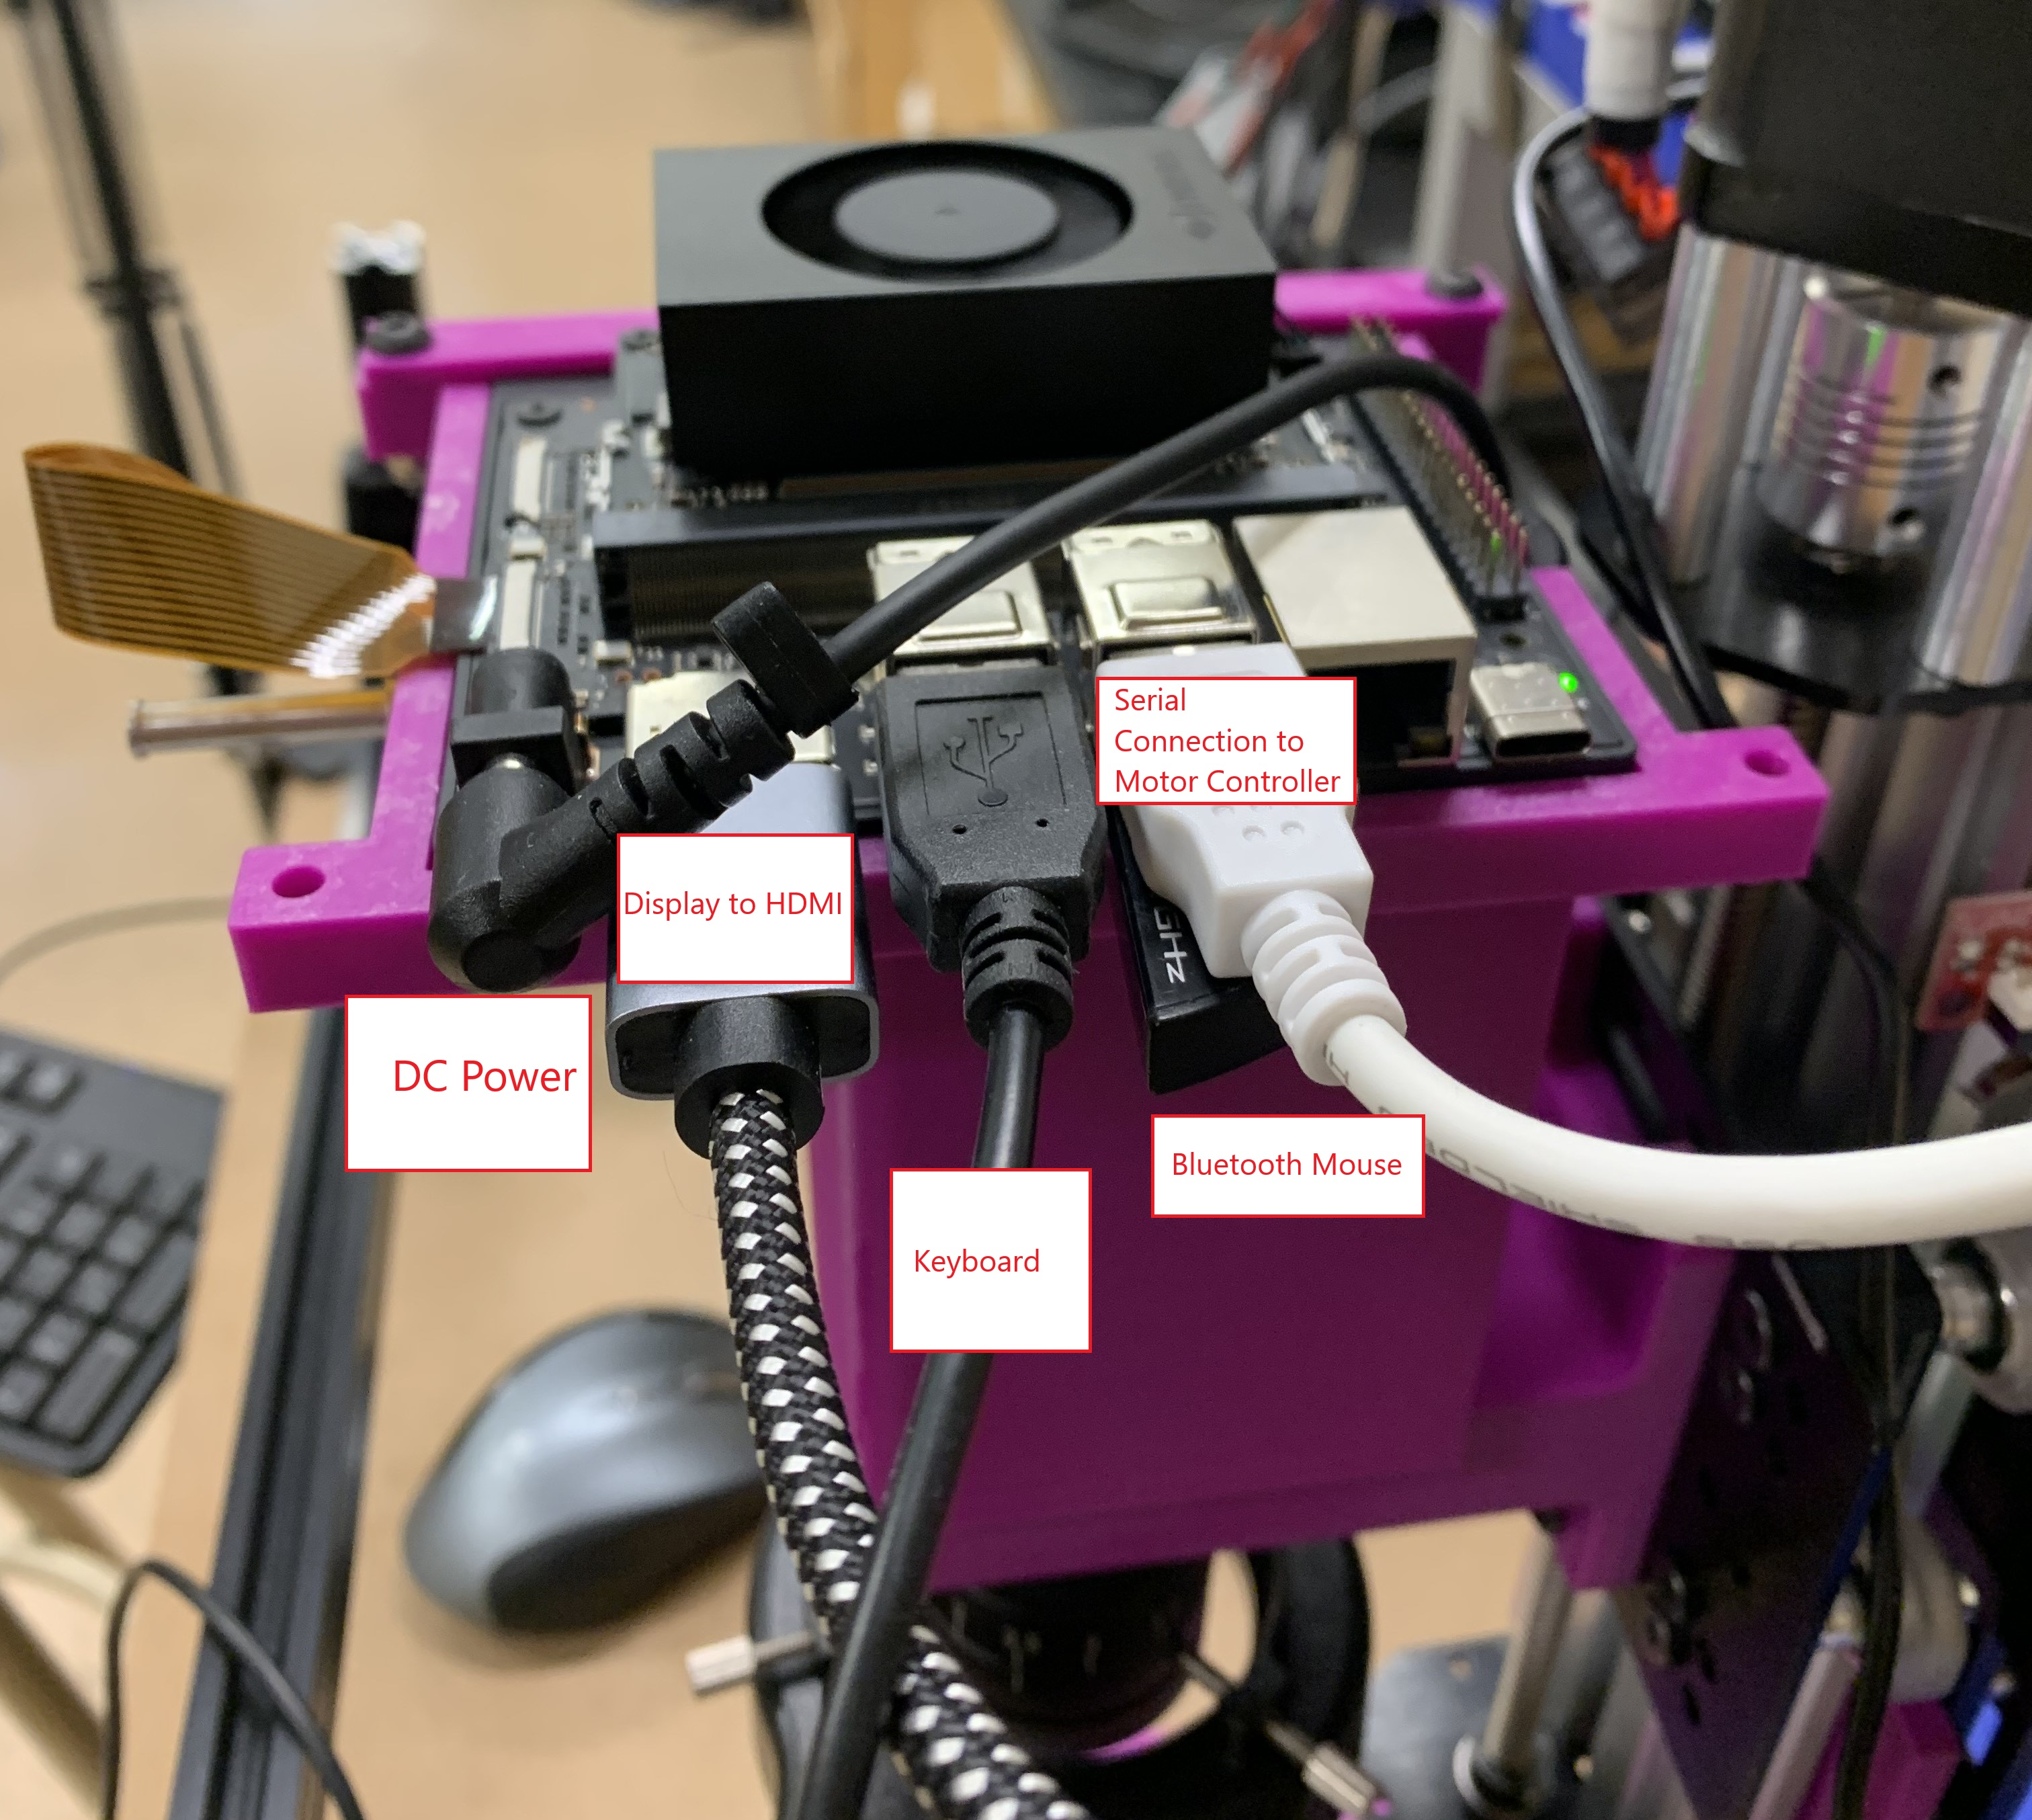
\includegraphics[width=\linewidth]{../content/jetson.jpg}
        \caption{Jetson Orin Nano with all the ports connected.}
        \label{fig:jetson1}
    \end{figure}

    \begin{figure}
        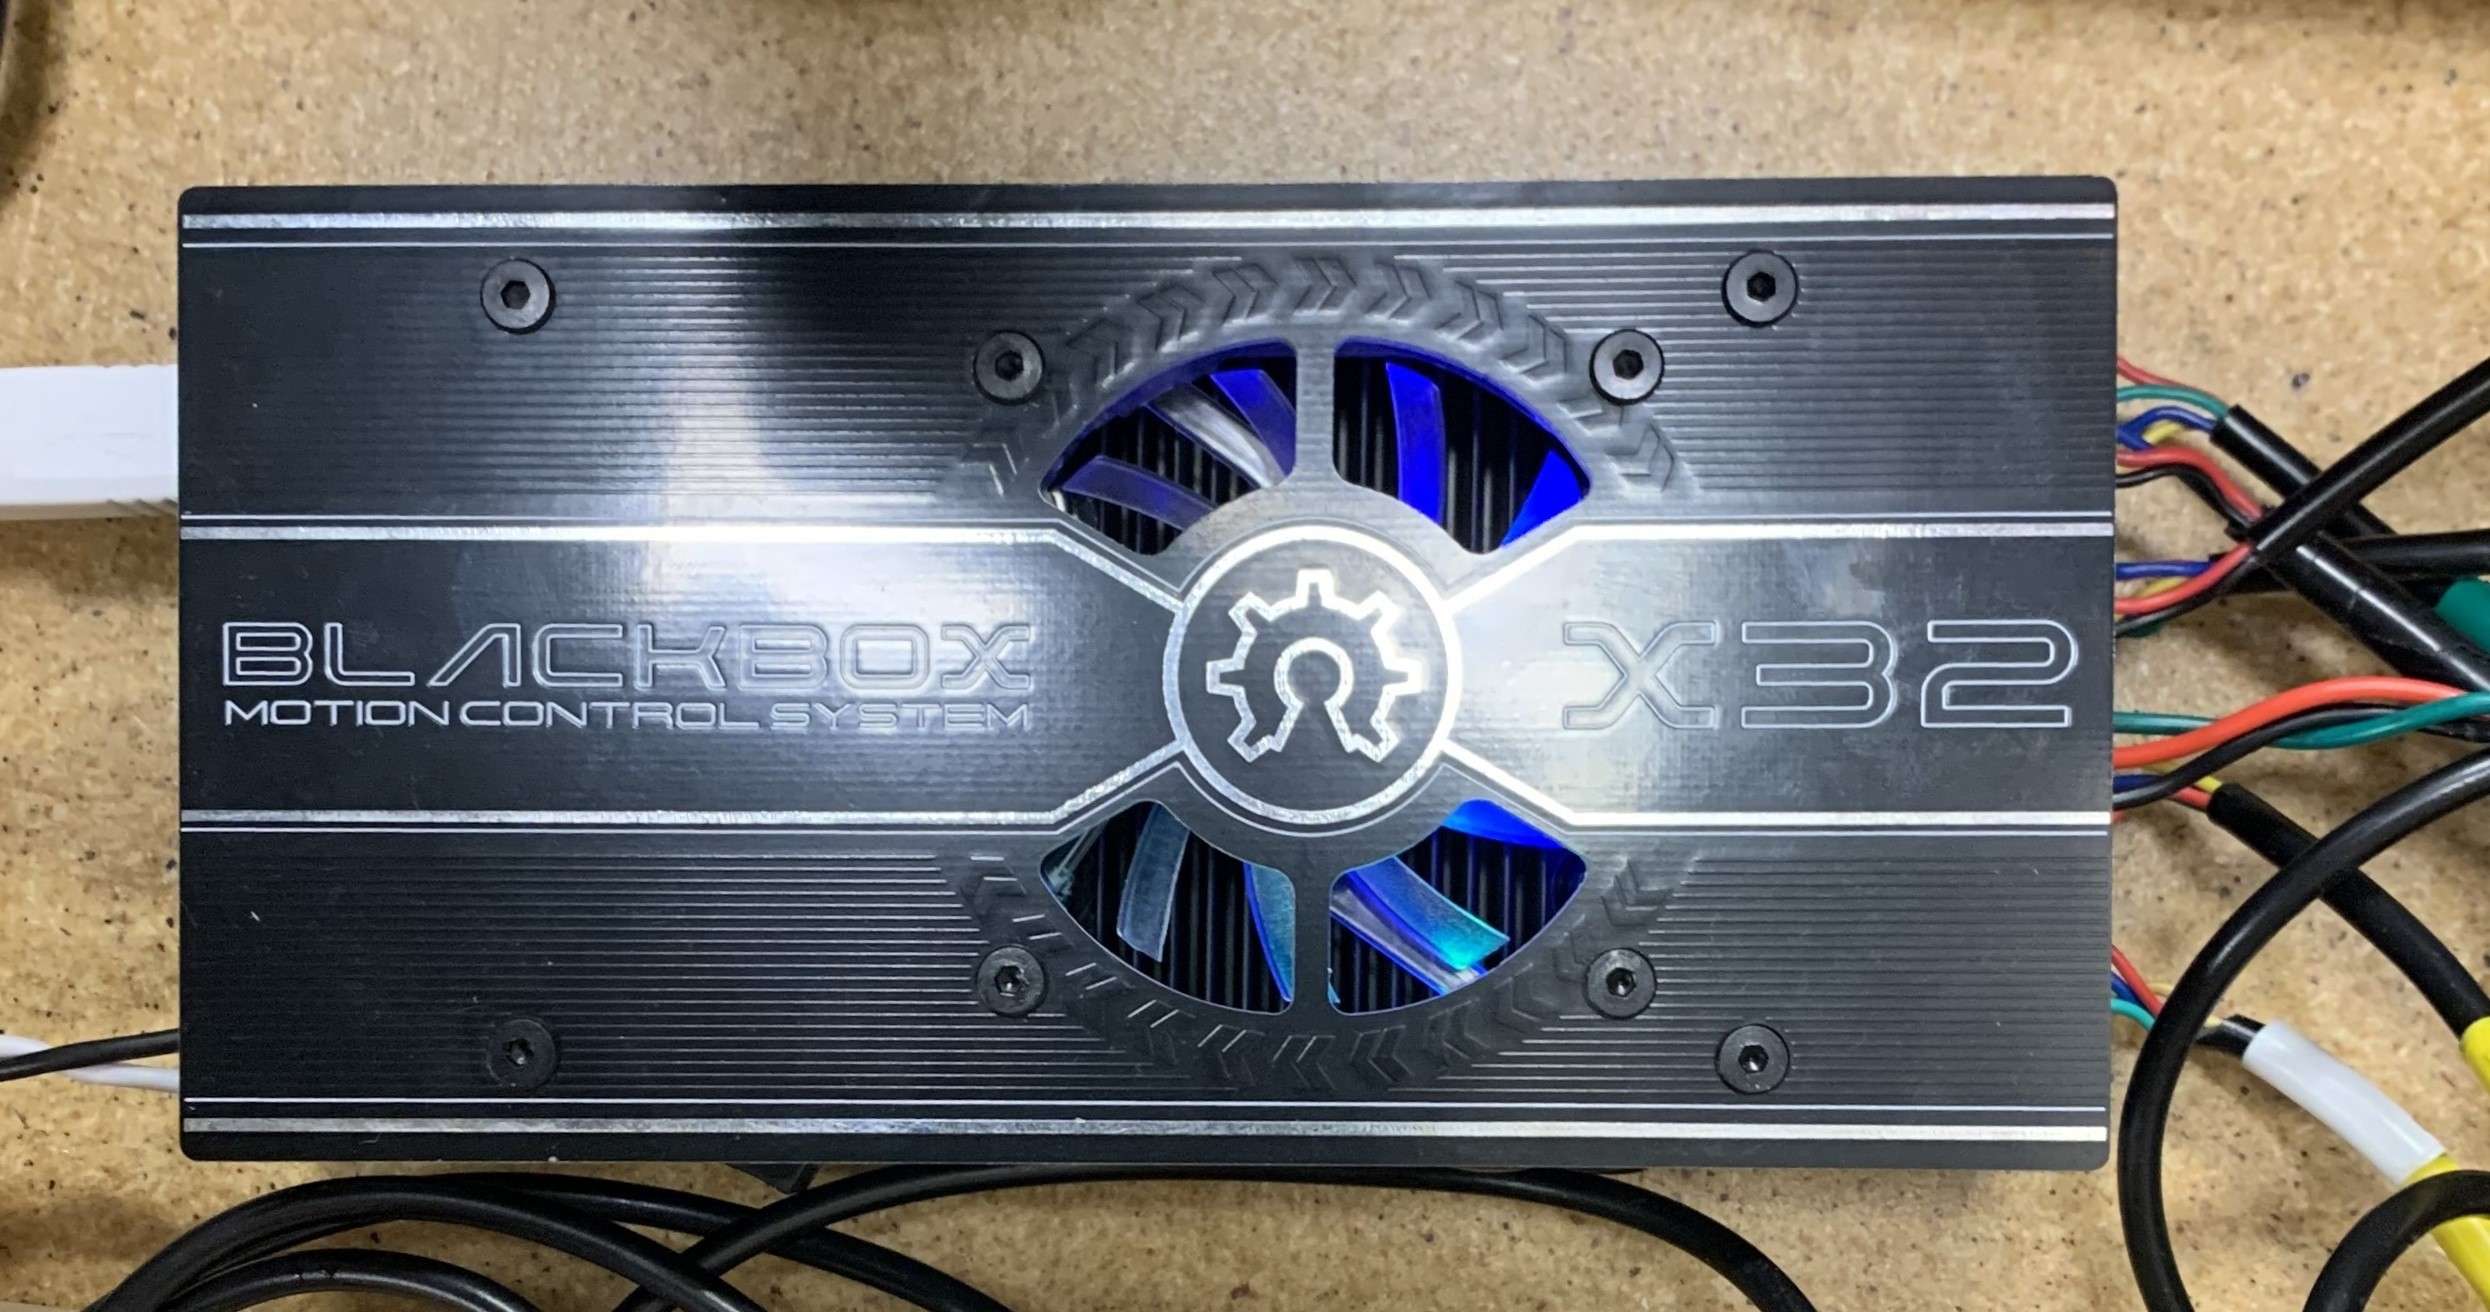
\includegraphics[width=\linewidth]{../content/motor_controller.jpg}
        \caption{Blackbox X32 Motor Controller from above.}
        \label{fig:controller1}
    \end{figure}

    \begin{figure}
        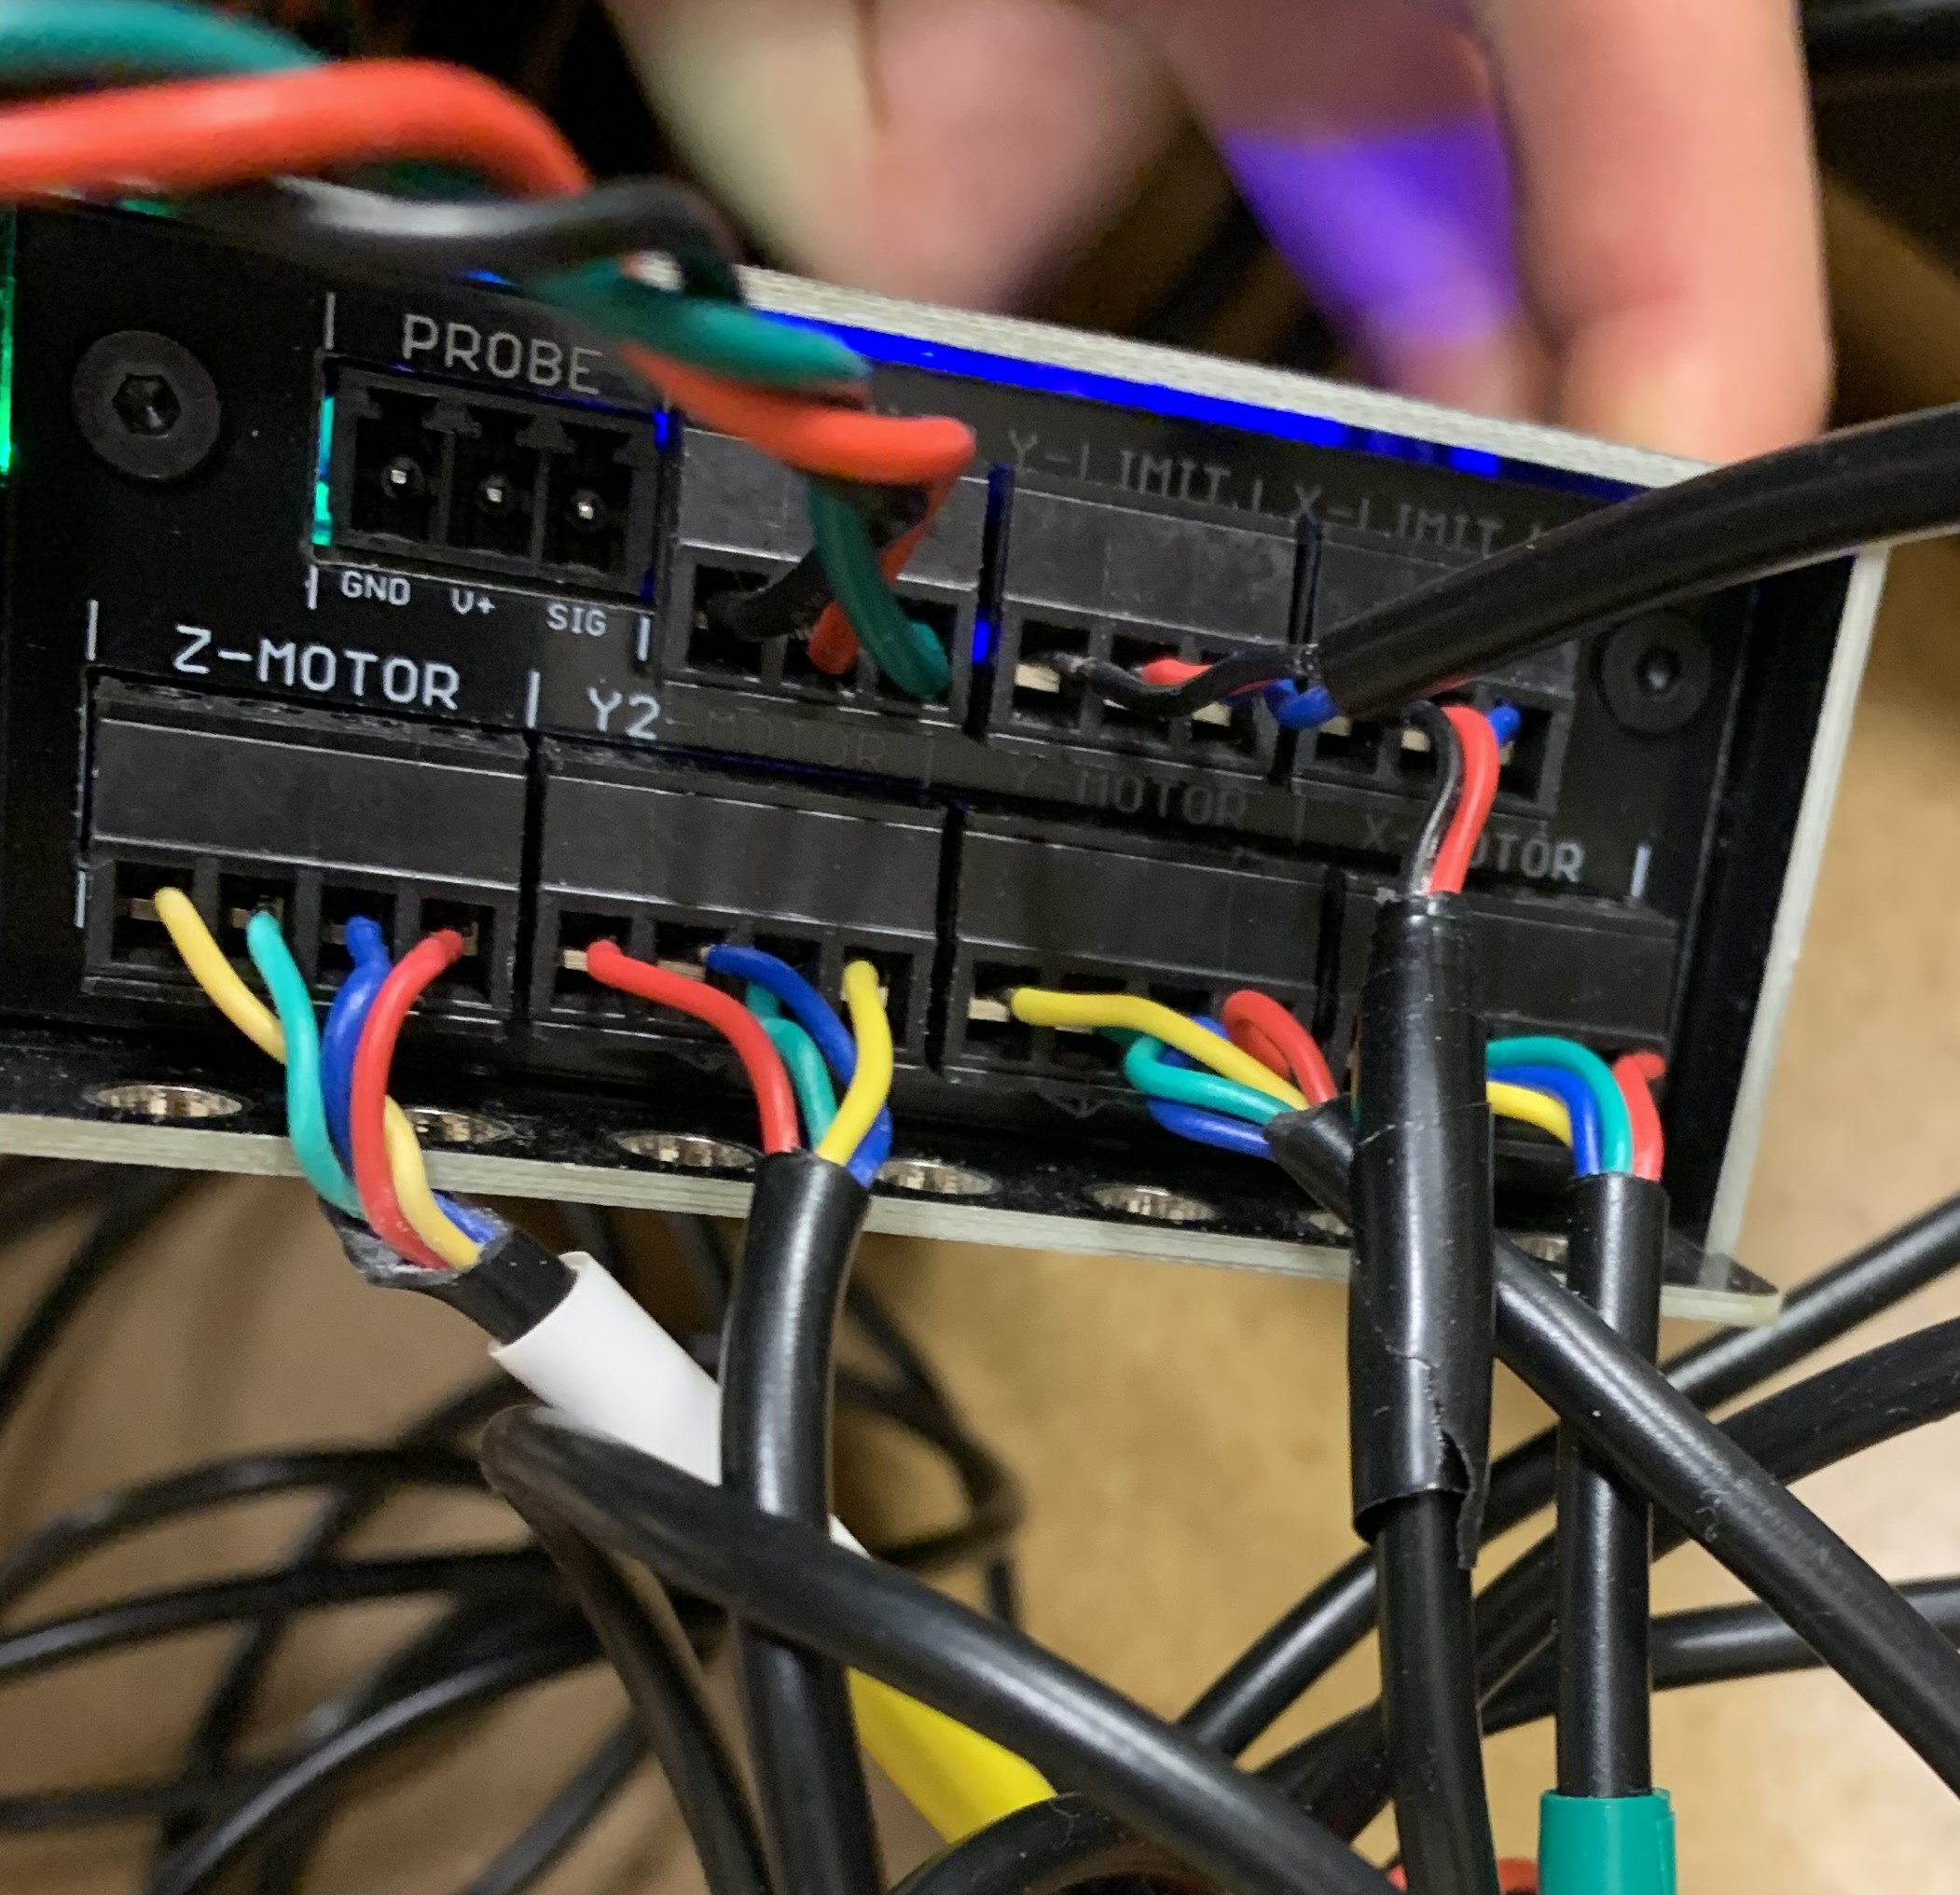
\includegraphics[width=\linewidth]{../content/motor_controller_connections.jpg}
        \caption{Blackbox X32 Motor Controller fully connected ports.}
        \label{fig:controller2}
    \end{figure}

    \begin{figure}
        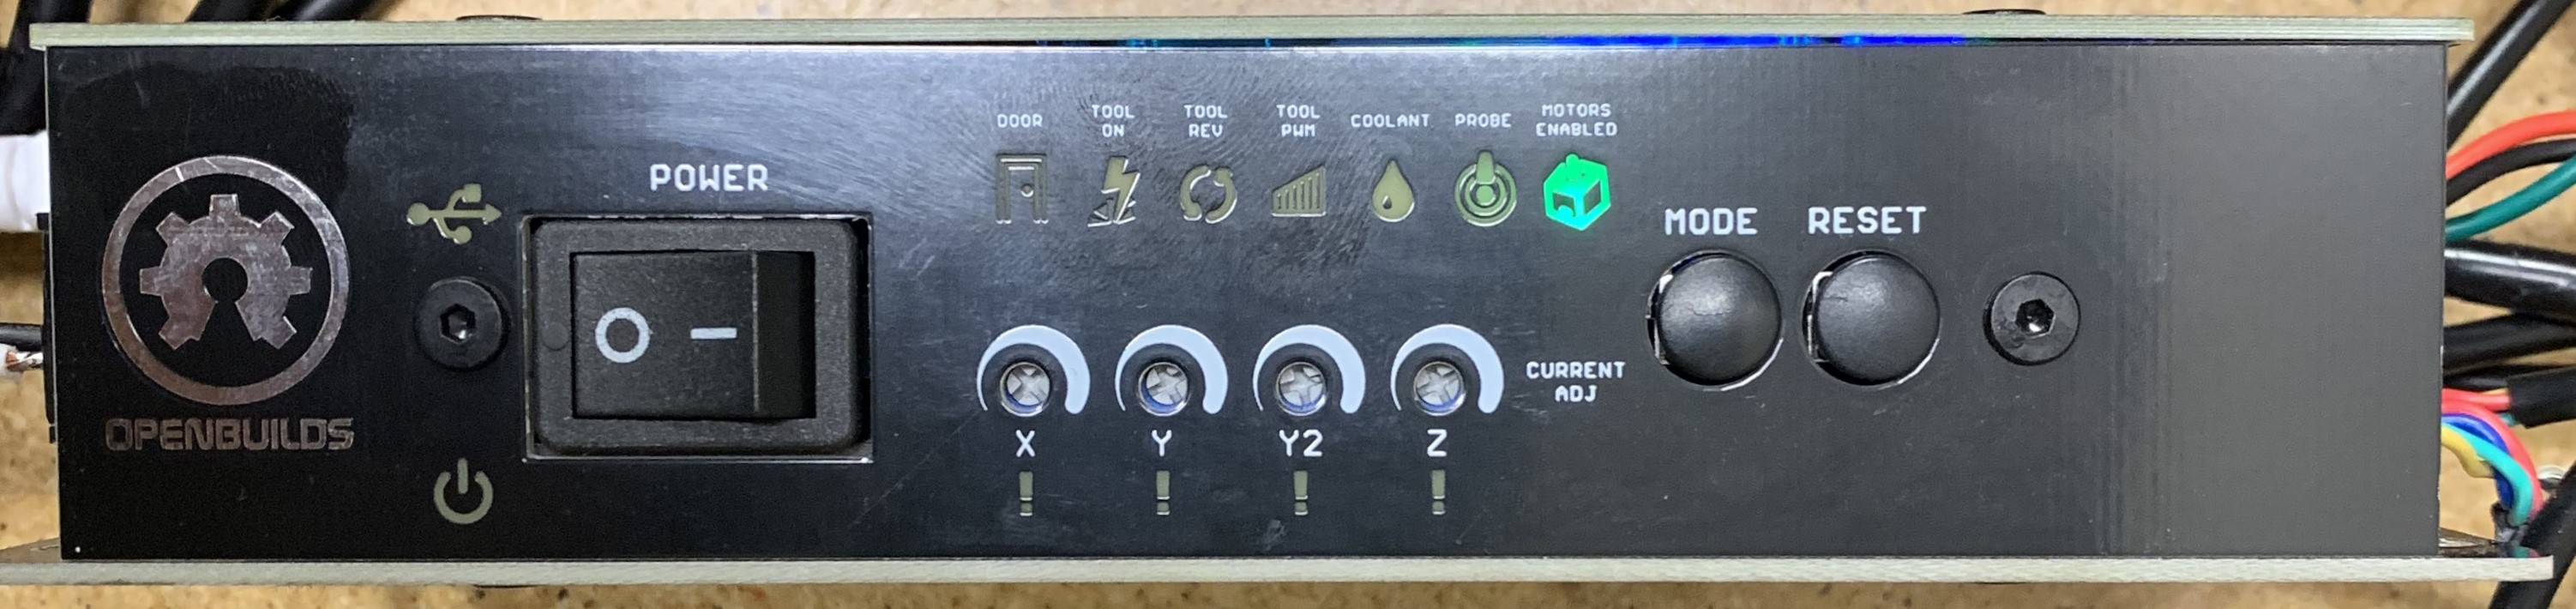
\includegraphics[width=\linewidth]{../content/motor_controller_buttons.jpg}
        \caption{Blackbox X32 Motor Controller buttons.}
        \label{fig:controller3}
    \end{figure}

    \begin{figure}
        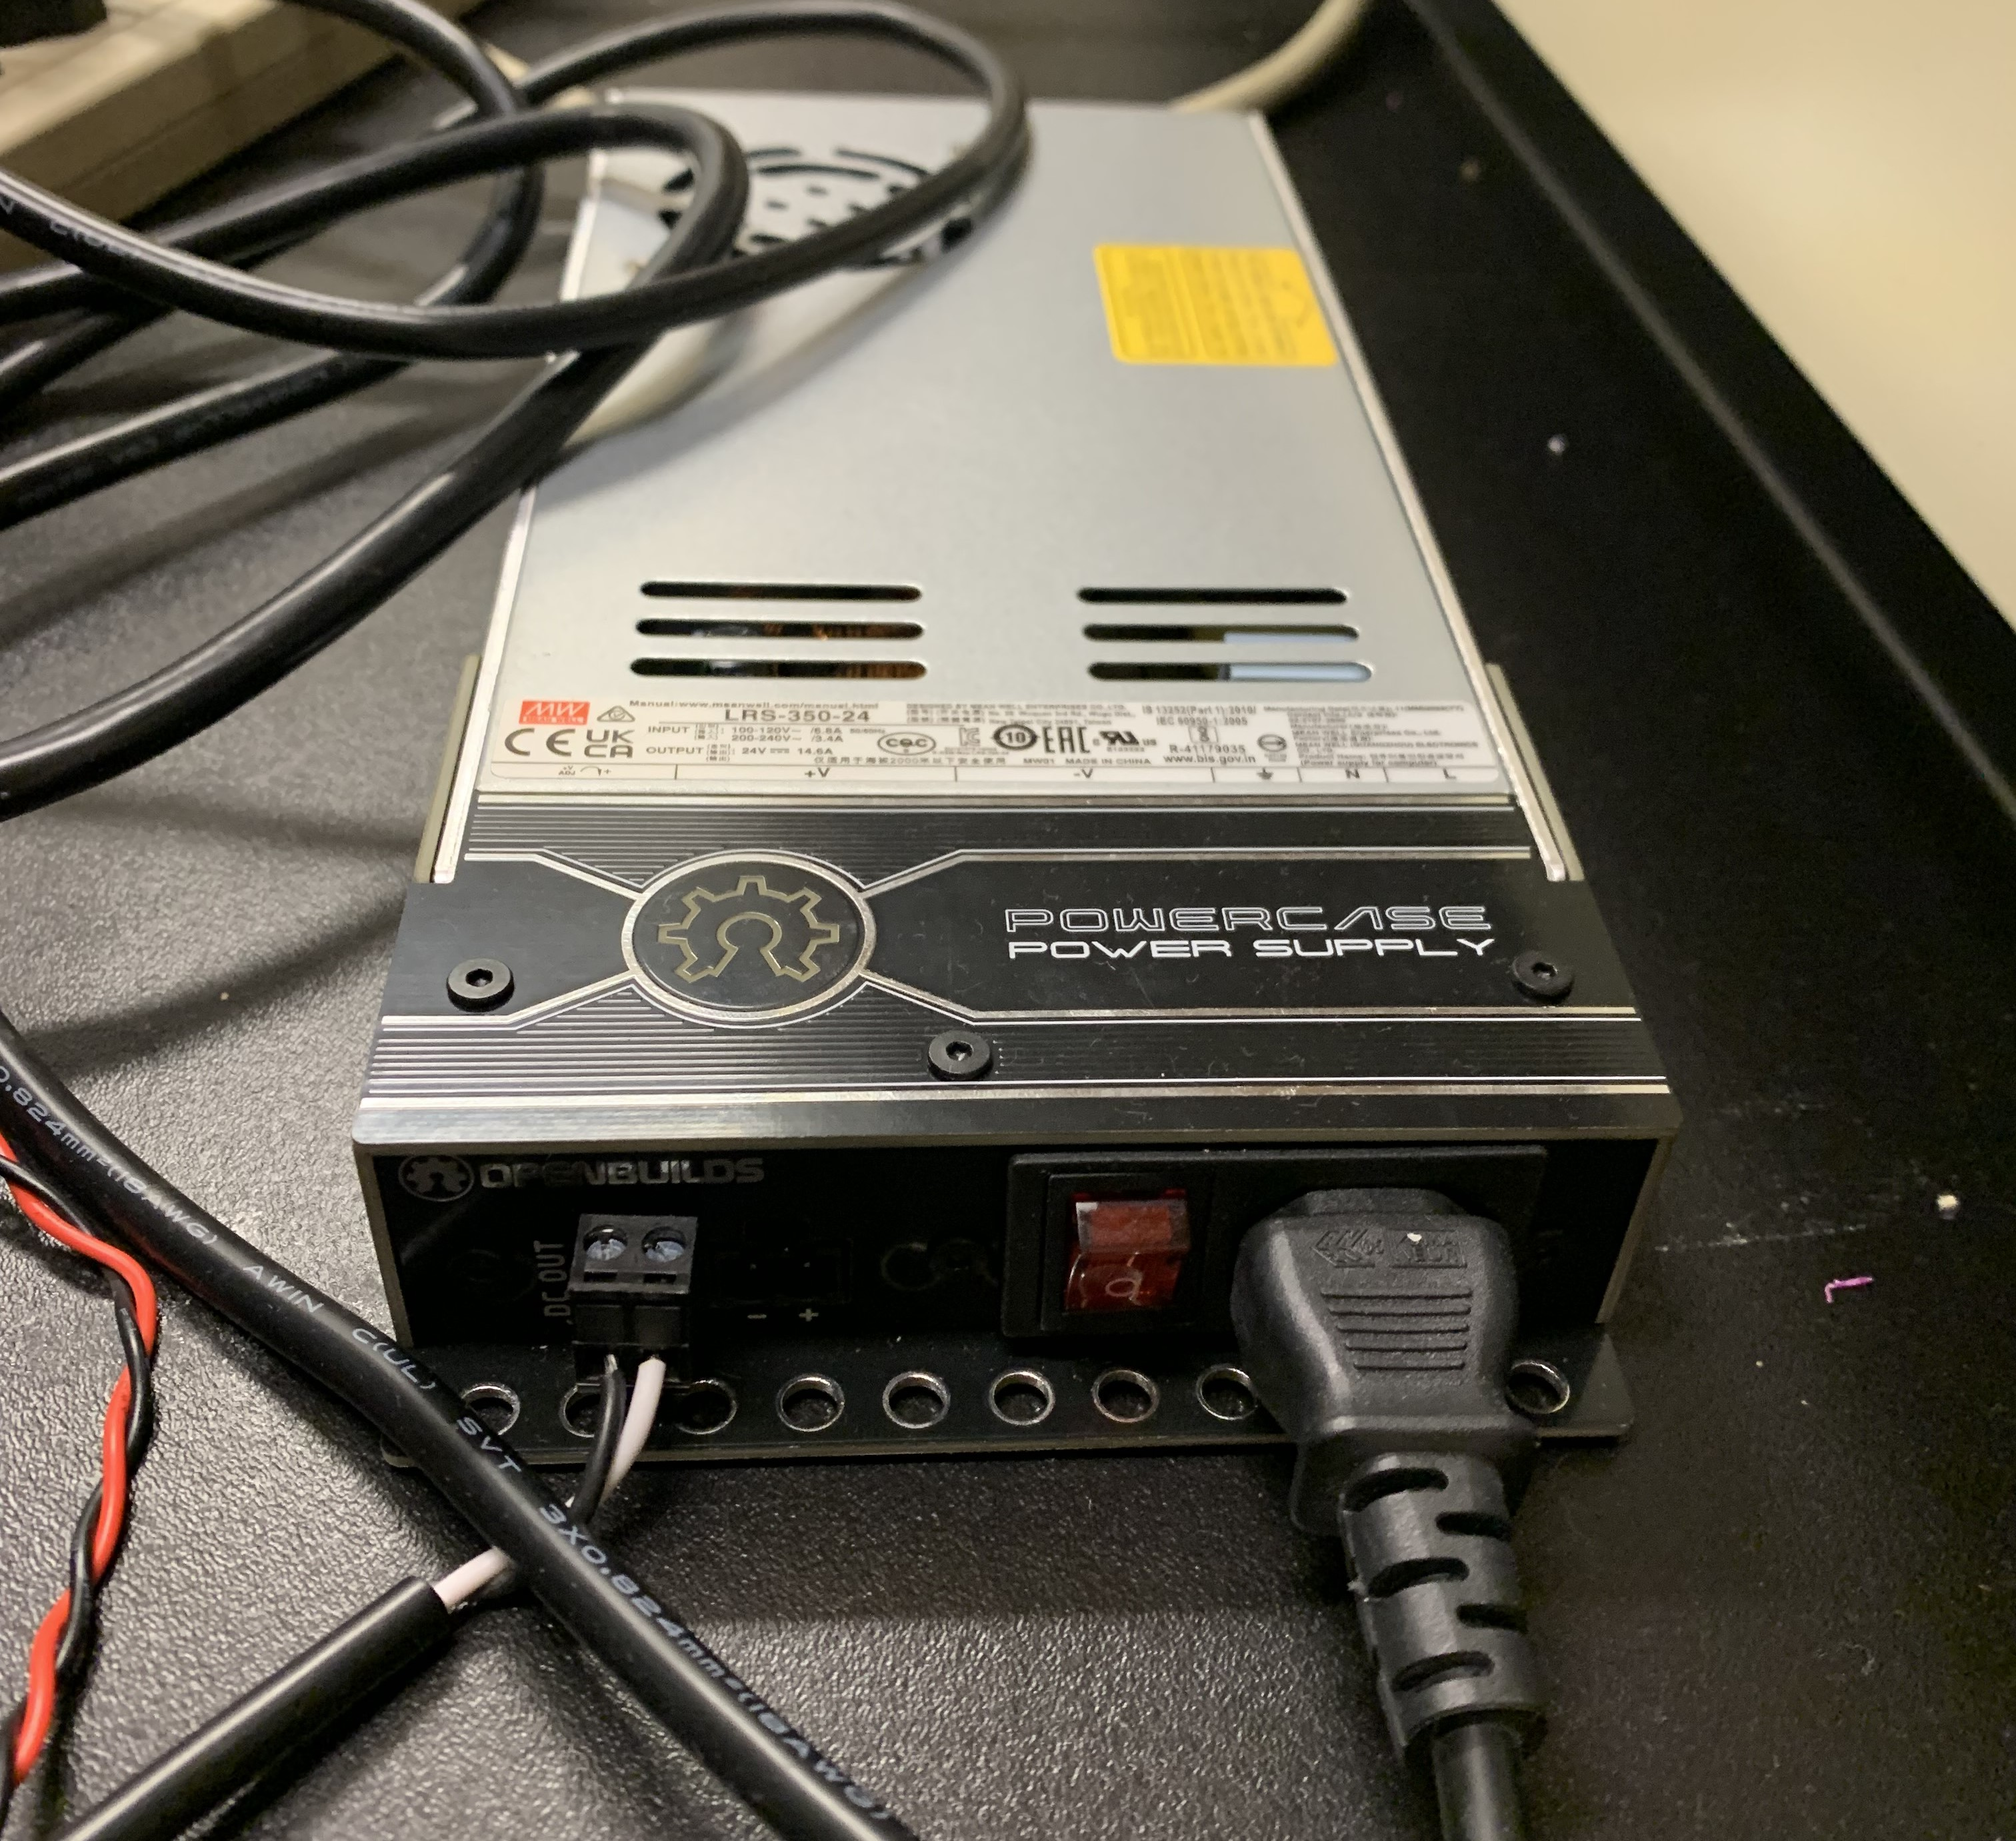
\includegraphics[width=\linewidth]{../content/power_supply.jpg}
        \caption{Power supply fully connected.}
        \label{fig:power1}
    \end{figure}

    \begin{figure}
        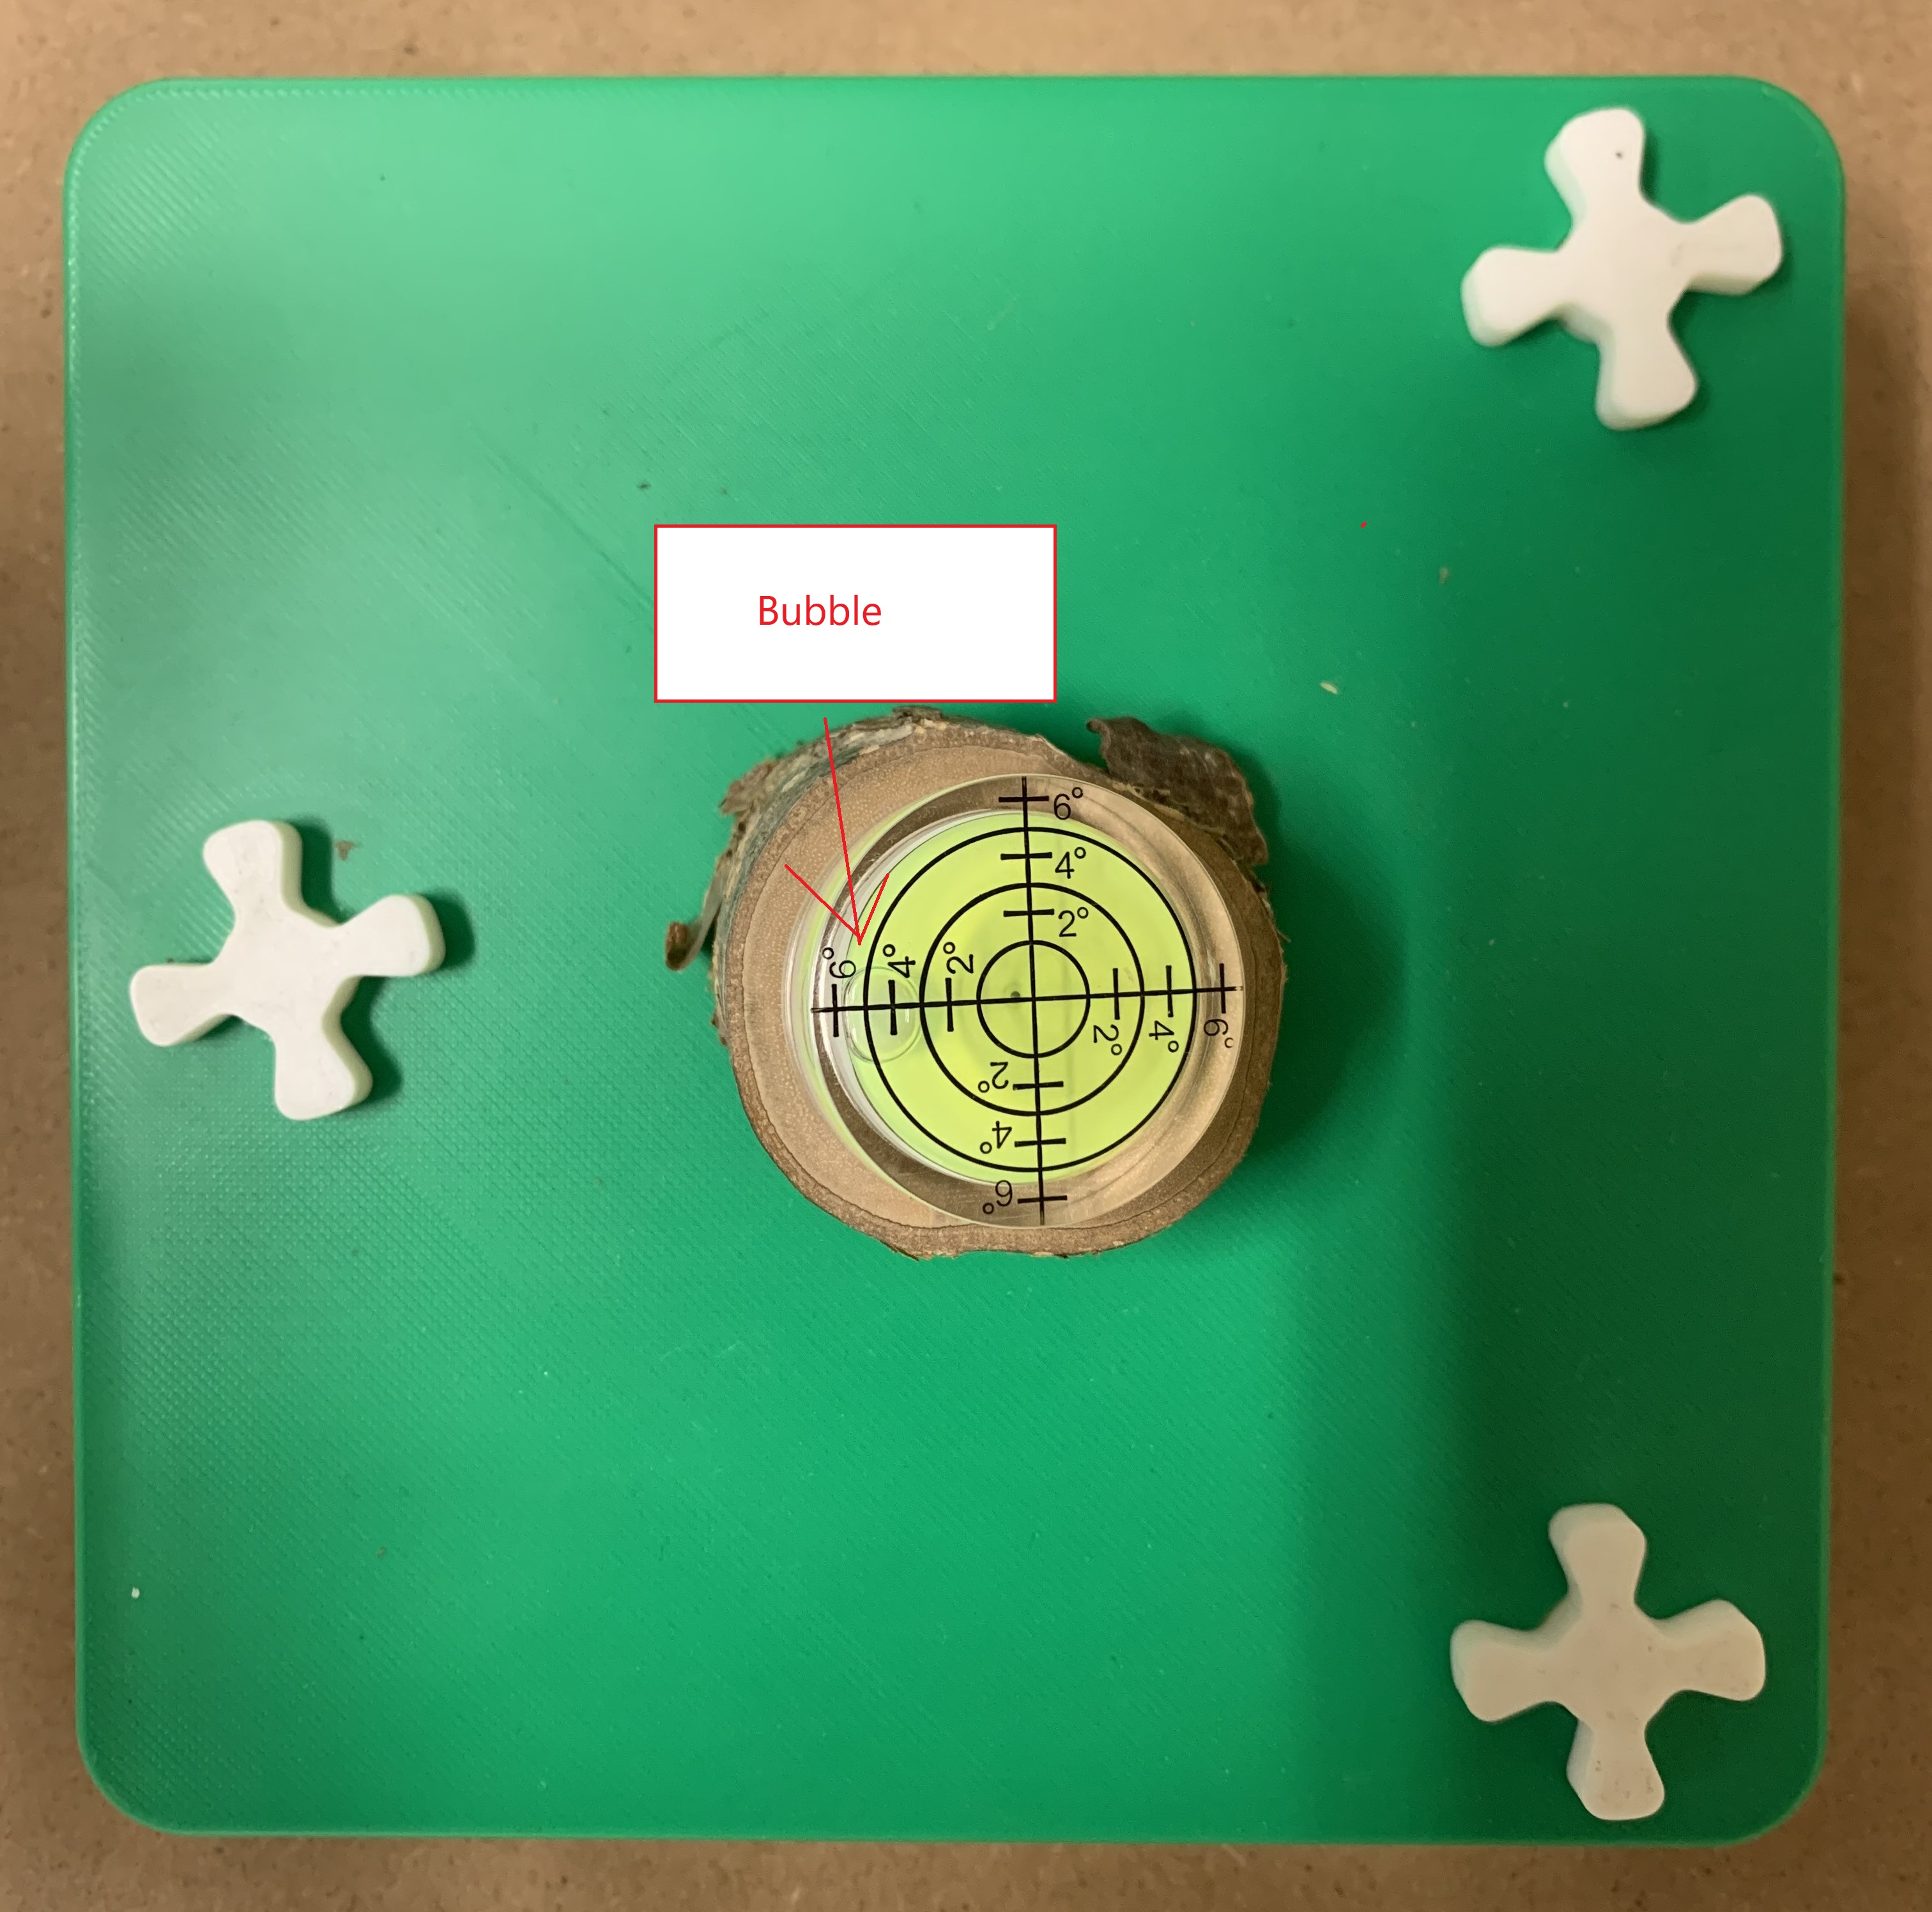
\includegraphics[width=\linewidth]{../content/sample_before_level.jpg}
        \caption{Cookie with the bubble of the level pointed directly towards the side of the table with one screw.}
        \label{fig:level1}
    \end{figure}

    \begin{figure}
        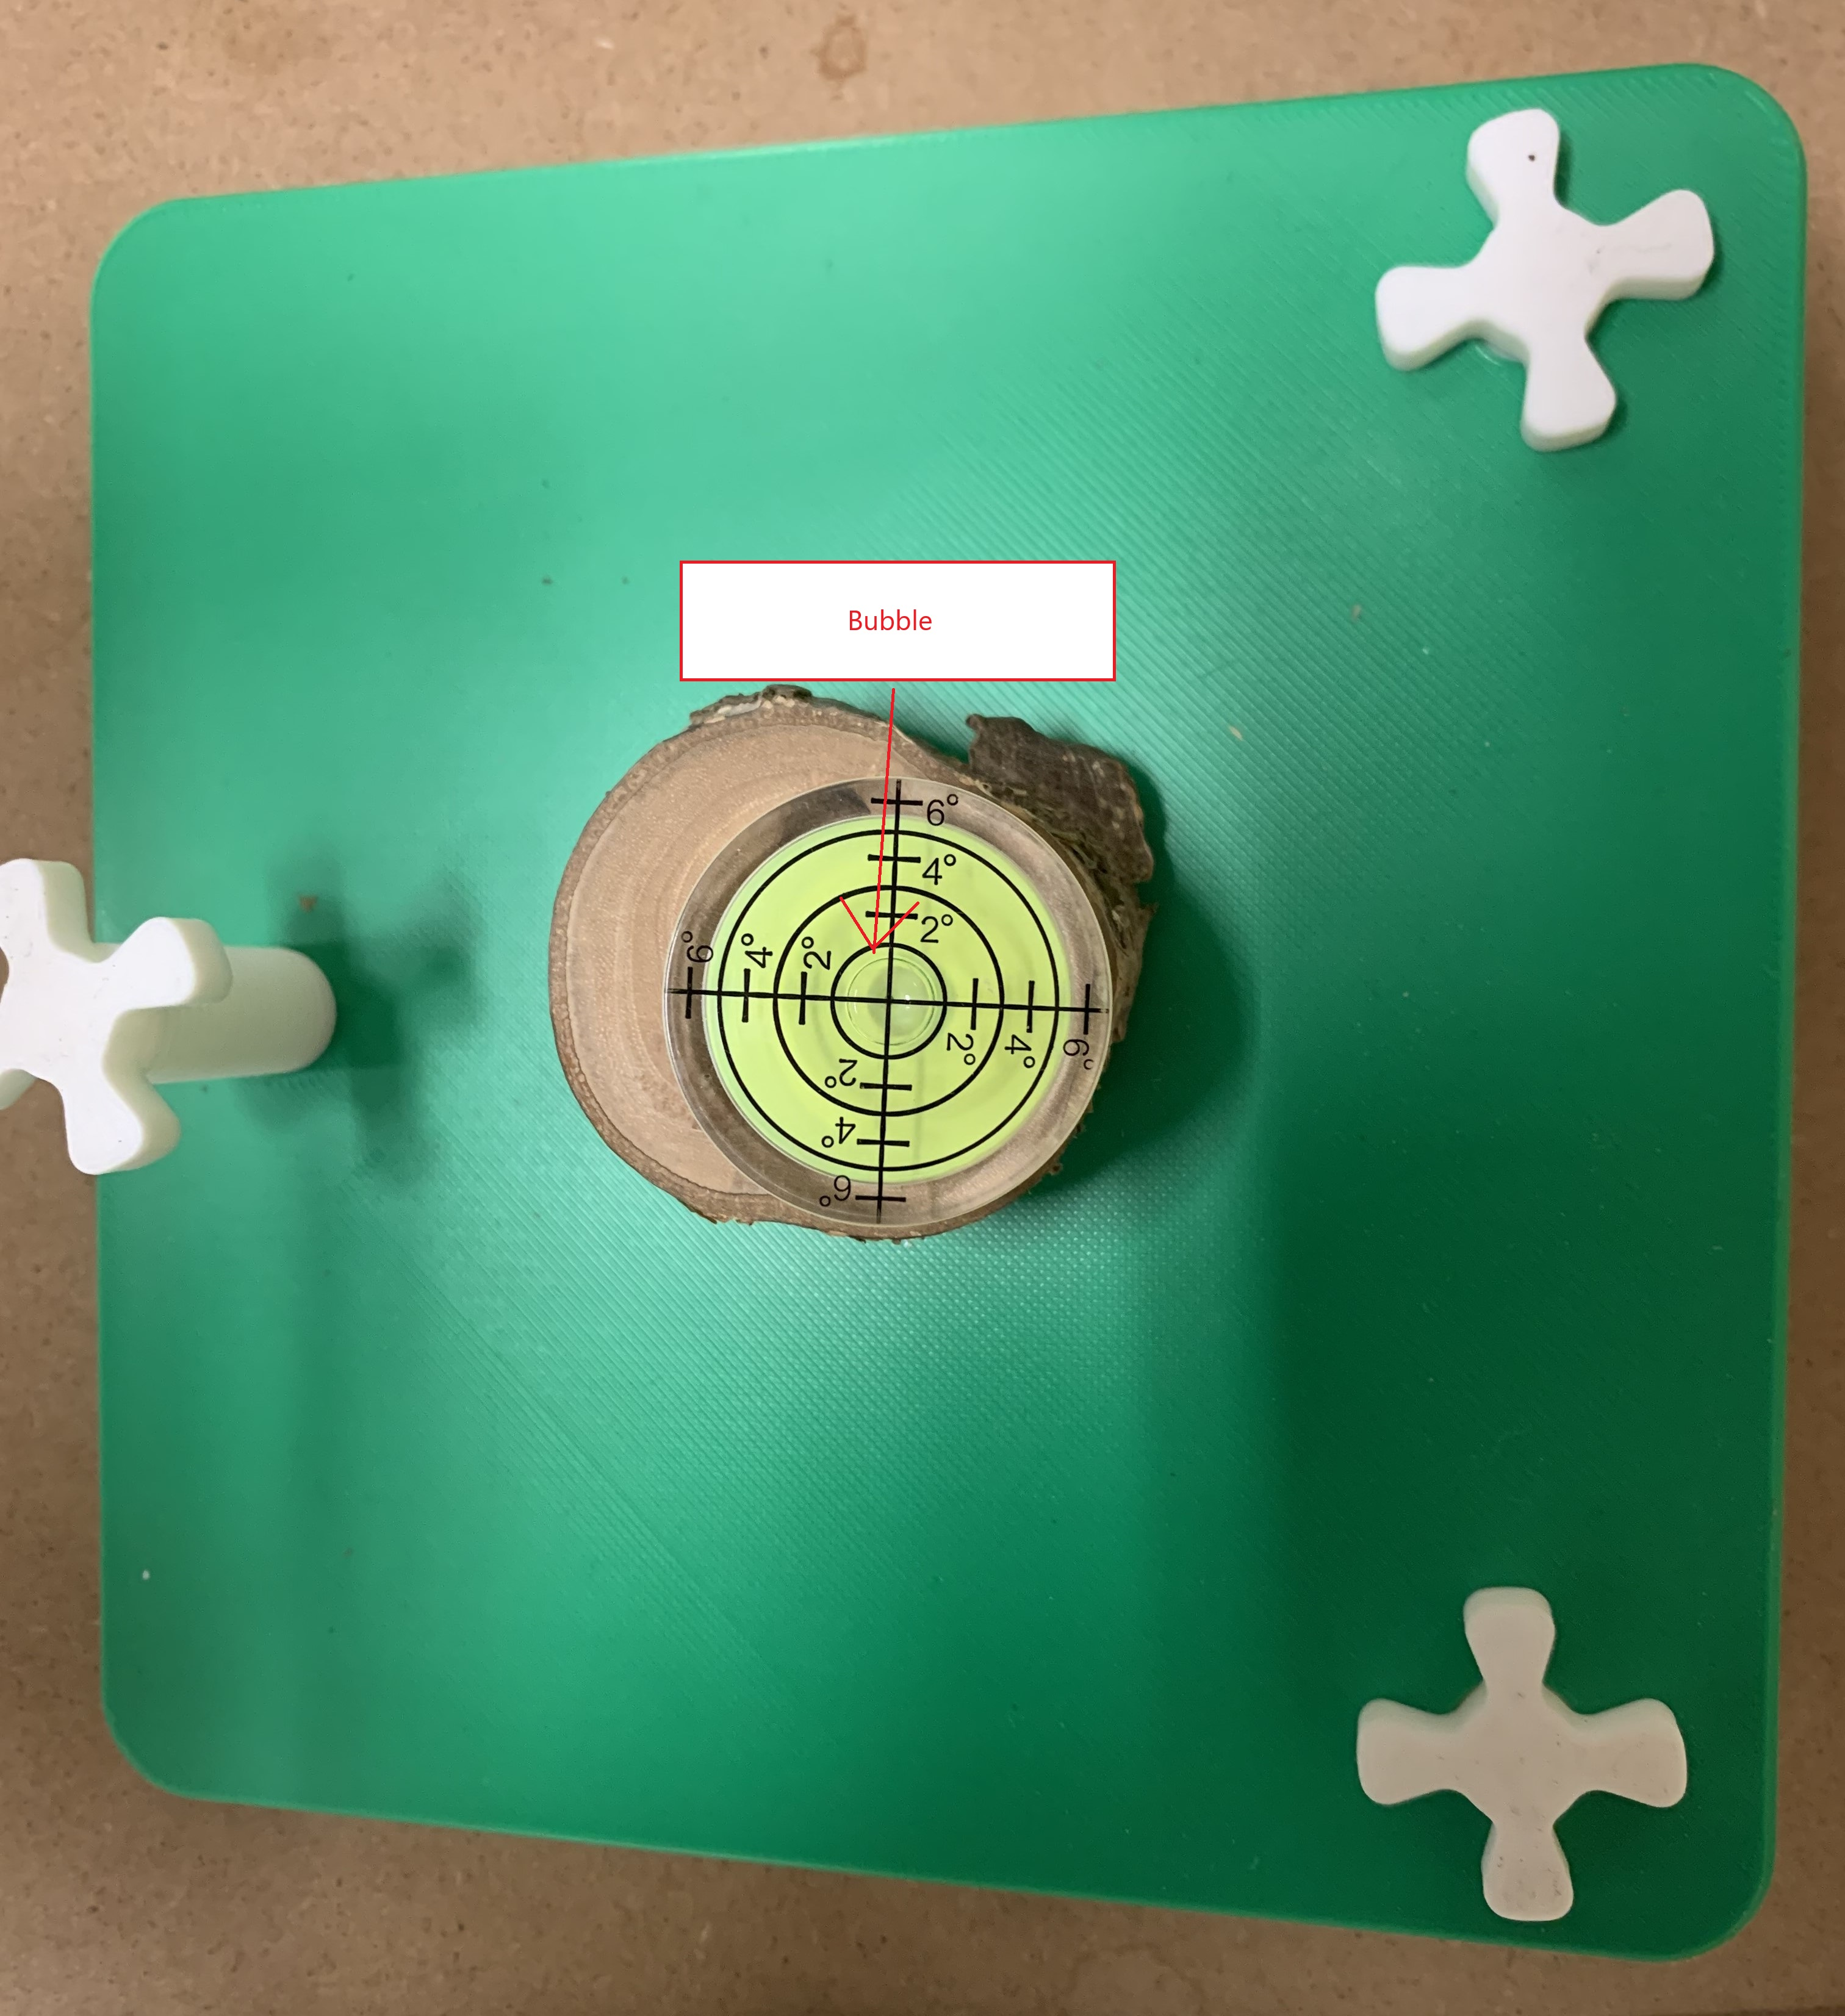
\includegraphics[width=\linewidth]{../content/sample_levelled.jpg}
        \caption{Cookie with the bubble of the level centered.}
        \label{fig:level2}
    \end{figure}
    
    \begin{figure}
        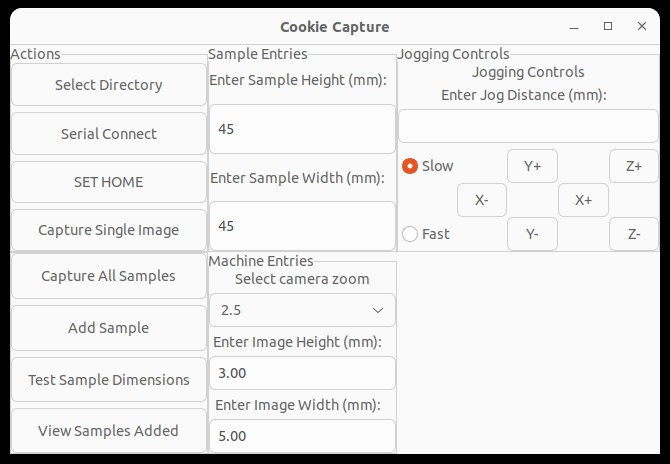
\includegraphics[width=\linewidth]{../content/gui.jpg}
        \caption{Default GUI appearance after launching.}
        \label{fig:gui1}
    \end{figure}
    
    \begin{figure}
        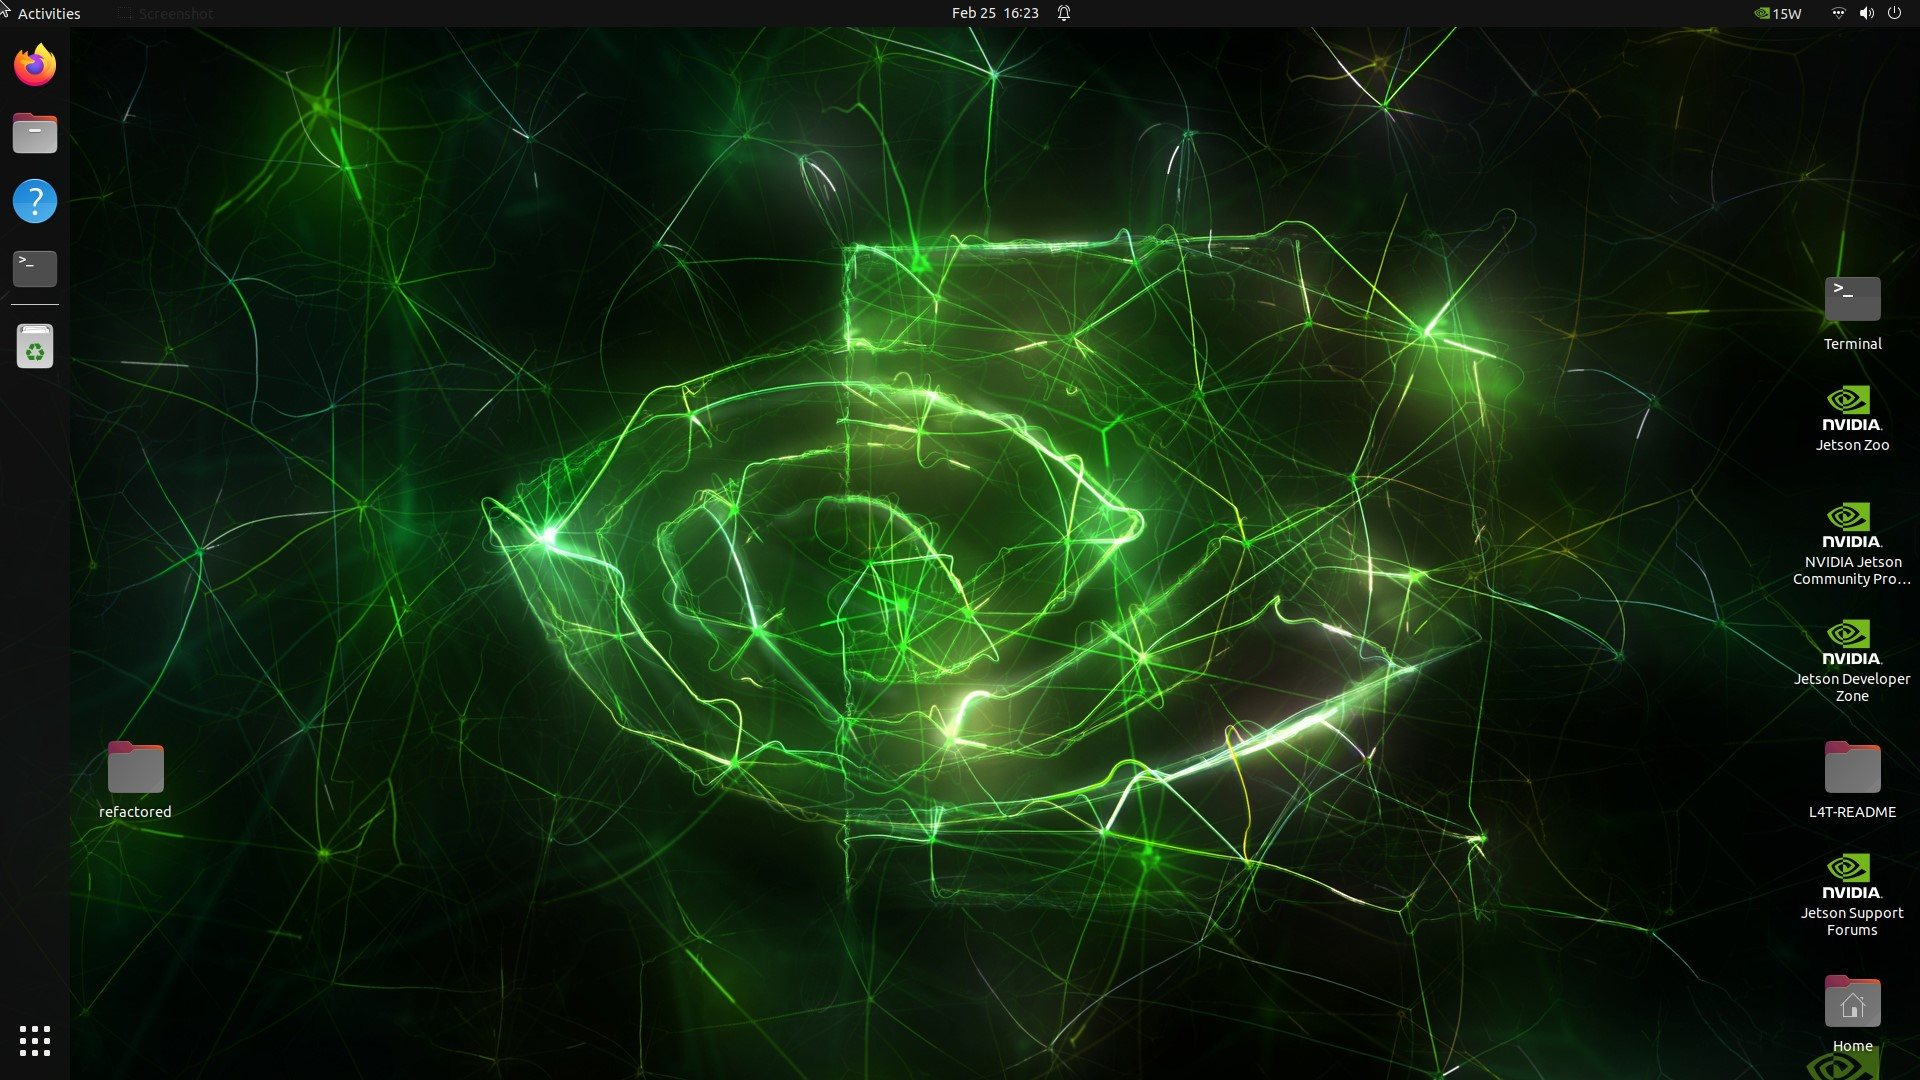
\includegraphics[width=\linewidth]{../content/background.jpg}
        \caption{Background after logging into the Jetson.}
        \label{fig:background1}
    \end{figure}
    
    \begin{figure}
        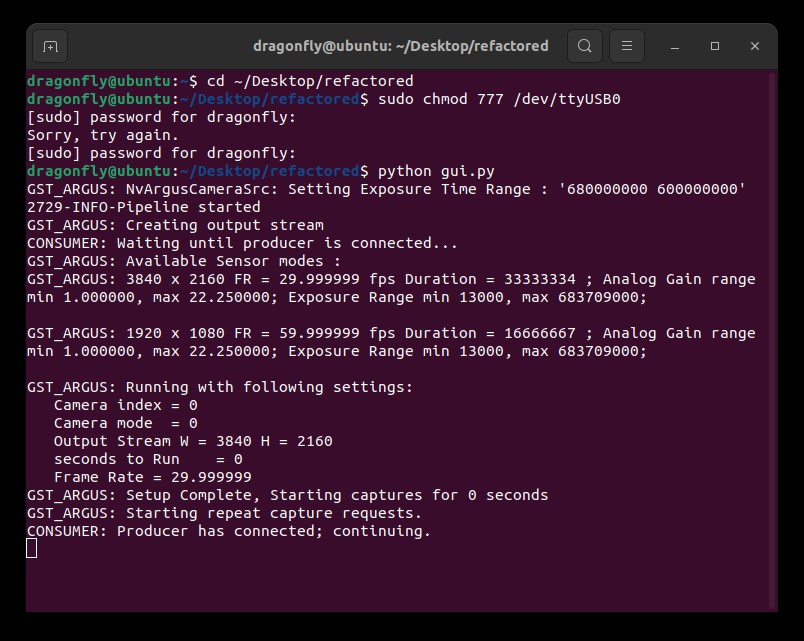
\includegraphics[width=\linewidth]{../content/terminal_commands.jpg}
        \caption{Background after logging into the Jetson.}
        \label{fig:terminal1}
    \end{figure}

\end{outline}
\end{document}